\section{GRID Plot Grid Toggle Function}

\subsection{Usage}

Toggles the drawing of grid lines on the currently active plot.  The
general syntax for its use is
\begin{verbatim}
   grid(state)
\end{verbatim}
where \verb|state| is either
\begin{verbatim}
   grid('on')
\end{verbatim}
to activate the grid lines, or
\begin{verbatim}
   grid('off')
\end{verbatim}
to deactivate the grid lines.  If you specify no argument then
\verb|grid| toggles the state of the grid:
\begin{verbatim}
   grid
\end{verbatim}
You can also specify a particular axis to the grid command
\begin{verbatim}
   grid(handle,...)
\end{verbatim}
where \verb|handle| is the handle for a particular axis.
\subsection{Example}

Here is a simple plot without grid lines.
\begin{verbatim}
--> x = linspace(-1,1);
--> y = cos(3*pi*x);
--> plot(x,y,'r-');
\end{verbatim}


\centerline{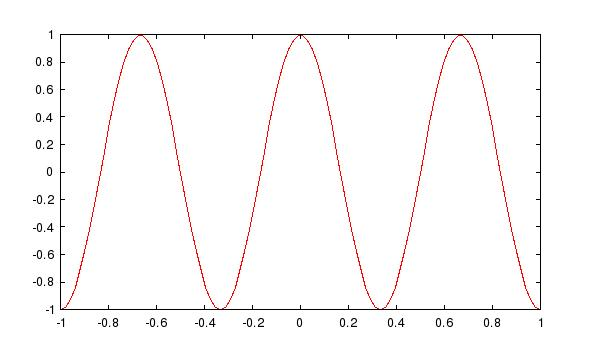
\includegraphics[width=8cm]{grid1}}


Next, we activate the grid lines.
\begin{verbatim}
--> plot(x,y,'r-');
--> grid on
\end{verbatim}


\centerline{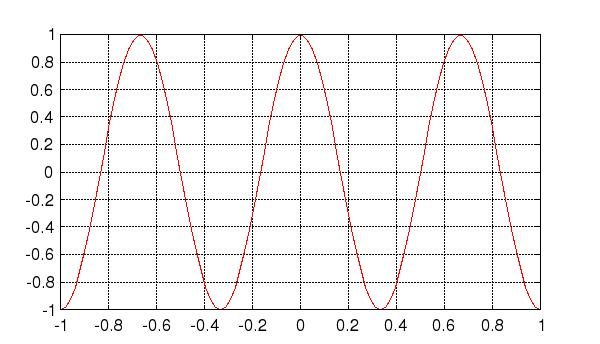
\includegraphics[width=8cm]{grid2}}

